\chapter{Implementation}\label{chap:Implementation}

In this section, we will discuss the implementation of each of the components of libbind. The workflow/usage is covered separately in Chapter~\ref{chap:Workflow}. Any major deviations from what has been covered in Design and Architecture will be highlighted.

\section{Binary Abstraction Layer}

The binary abstraction layer was originally designed to act as a bridge between the components and the target file. Essentially, libbind encapsulates a binary file in an internal structure called a \emph{bin\_file}. A \emph{bin\_file} contains two important elements: the BFD abstraction of a binary and its corresponding CFG (which is generated by the static analysis engine). In general, when a component needs to read information about the binary, it will read from the generated CFG. As we have seen, writing to the binary is equivalent to modifying the CFG. After a change to the CFG occurs, this change is flushed to the underlying binary through the BFD object. This was the original concept but it had to be modified to work in practice. Figure~\ref{fig:BAL_Attempt1} illustrates the original approach to creating the binary abstraction layer.

\begin{figure}[H]
 \centering
 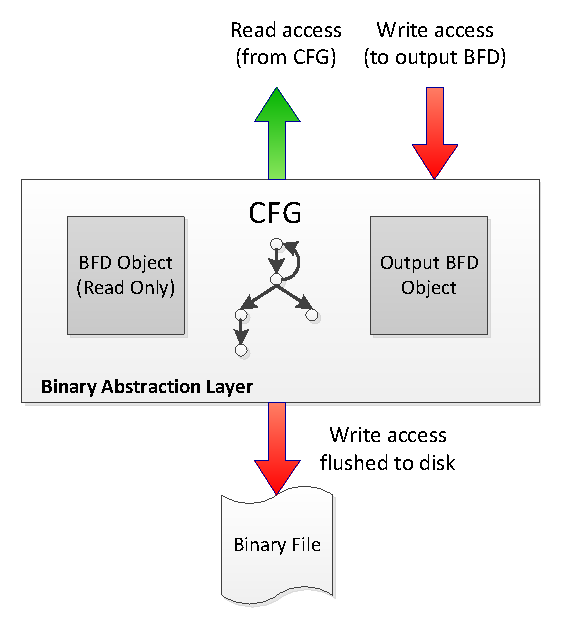
\includegraphics[scale=0.86]{Binary_Abstraction_Layer_Attempt1.pdf}
 \caption{The original approach for the binary abstraction layer. The read only BFD object is the abstraction of the original binary file. The CFG is generated from this BFD. Any changes need to be outputted to the output BFD independently.}
\label{fig:BAL_Attempt1}
\end{figure}

\subsection{Original Approach}

The problem with the original design was that it only encapsulated a single BFD object. With libbfd, it is possible to open a file in two ways:

\begin{enumerate}
\item An existing file can be opened with read-only access.
\item A \emph{new and empty} file can be opened with write access.
\end{enumerate}

This restriction of libbfd is by design, but does not make it ideal for patching. Tools such as \emph{ld} and \emph{objcopy} work well above libbfd because the files they output are written in a single pass. Although BFD is unsuitable for our usage, it is possible (albeit very awkward) to patch a binary file. Figure~\ref{fig:BAL_Approach1} illustrates the steps required to patch a file through libbfd:

\begin{figure}[H]
 \centering
 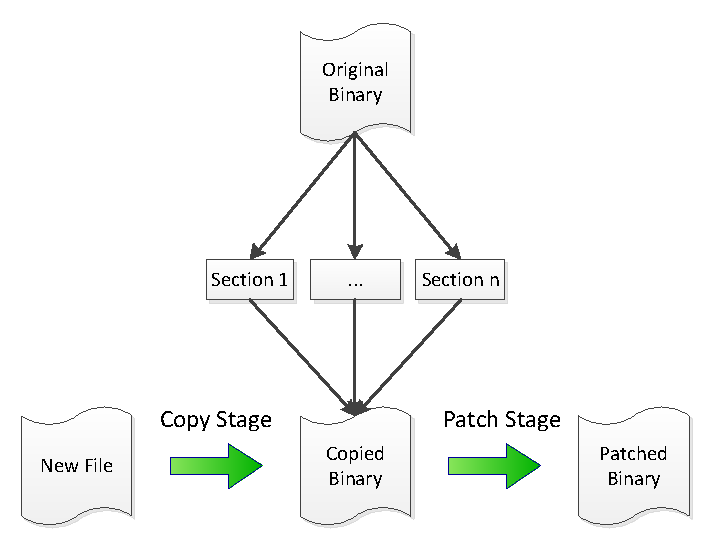
\includegraphics{Binary_Abstraction_Layer_Approach1.pdf}
 \caption{The process required to patch a file using libbfd.}
\label{fig:BAL_Approach1}
\end{figure}

The abstraction used within BFD is that an object file has:

\begin{itemize}
\item A header
\item A number of sections containing raw data (this data could represent code)
\item A set of relocations
\item Symbol information
\end{itemize}

As illustrated, patching a binary file with libbfd works through a series of steps:

\begin{enumerate}
\item The original binary must first be opened with read access.
\item A new BFD (which starts off empty) is created. The original binary is then reconstructed in this BFD by extracting the four different types of content (as defined above) and copying them. This reconstruction all happens in memory.
\item Before the new BFD object is flushed to disk, the user is able to perform patches by editing the contents of sections.
\item After all patches are performed, the BFD object is flushed to disk. If more modifications are needed after this, the entire process has to be restarted.
\end{enumerate}

In terms of the implementation of this algorithm, the first two stages are essentially what objcopy does. Our implementation of static patching re-uses the objcopy code for the decomposition and reconstruction stage. The rest of the algorithm is trivial to implement. However, there are two drawbacks with this method:

\begin{enumerate}
\item The part of the code re-used from objcopy is large, approximately 1.5 KLOC.
\item BFD is merely an abstraction over many file formats. This means that it represents a more generalised abstract format. Unfortunately, it does not encapsulate all the information required for the full reconstruction of a binary. In order to obtain this information, the code relies on a dependency with the file format and ends up calling functions in libelf.
\end{enumerate}

\subsection{Final Approach}

Given the disadvantages of using the method from the original approach, there is no reason to use BFD to perform the patching. The method is overly complicated and more error-prone simply because of the amount of code that has to be written to perform a patch. Since a dependency on libelf is unavoidable, we can re-implement the solution by using libelf directly and save the hassle of forcing libbfd to do something it was not designed for. In terms of the binary abstraction layer, this means that we modify write accesses to directly modify the disk version instead of through the BFD object as seen in Figure~\ref{fig:BAL_Final}:

\begin{figure}[H]
 \centering
 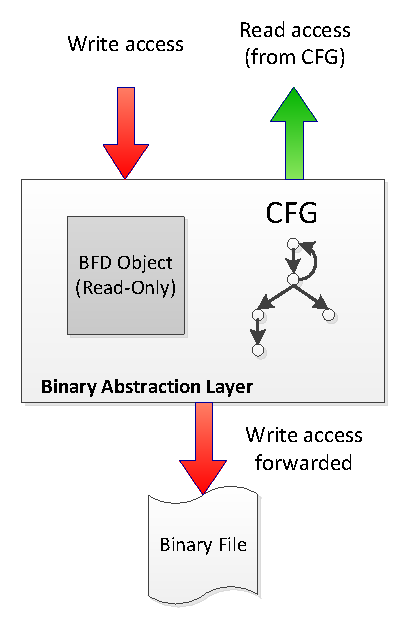
\includegraphics{Binary_Abstraction_Layer_Final.pdf}
 \caption{The final design for the binary abstraction layer. Read accesses are handled in the same way but in this design, we have removed the output BFD. Write accesses are alter the target binary file directly.}
\label{fig:BAL_Final}
\end{figure}
 
In the final implementation of the binary abstraction layer where libelf is used, the same result as with the original approach can be achieved in under 100 LOC. The method is fairly intuitive and the concept is visualised in Figure~\ref{fig:Loading_Binary}:
 
\begin{figure}[H]
 \centering
 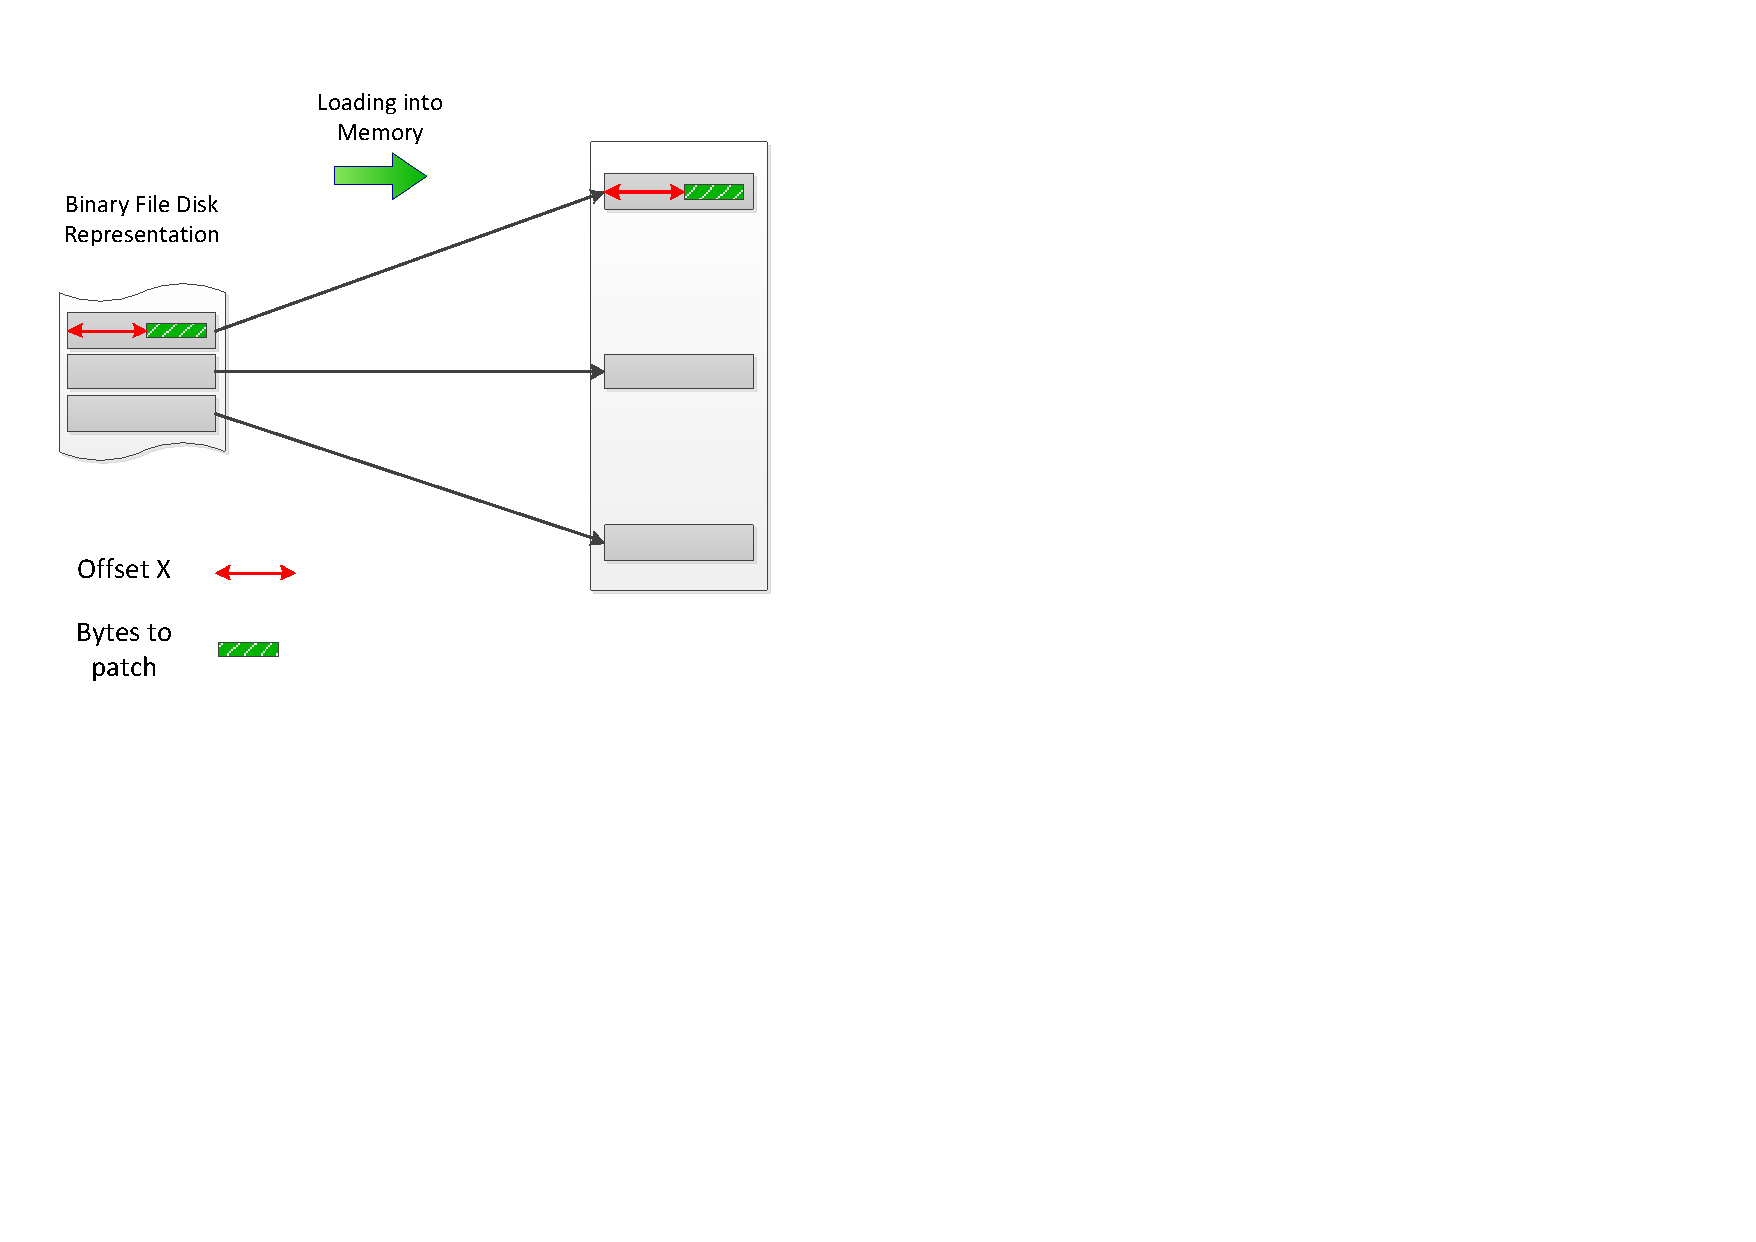
\includegraphics{Loading_Binary.pdf}
 \caption{The concept of how patching works in the final implementation. The most important idea here is that a section in the disk representation is preserved (not split) when it is mapped into memory. This means data that is at a certain offset into the section in the disk representation will be offset by the same amount after loaded into memory.}
\label{fig:Loading_Binary}
\end{figure}
\todo{add label for the loaded executable (memory)}
 
In libelf, similarly to libbfd, an executable contains a set of sections in which both code and data can reside. When the operating system loads the executable into memory, each section is based at some base address. We can reverse this to map a virtual memory address to a physical file offset. If a physical file offset can be found, the bytes can be patched as a regular file.

\begin{enumerate}
\item First, the section header of the executable is parsed with libelf. This allows us to obtain a set of sections and most importantly, for each section libelf can tell us three things:
  \begin{description}
  \item [Section size] The size of the section.
  \item [Section base address] The address that the section will be based at when the executable on disk is loaded into memory.
  \item [Section disk offset] The disk offset of the section.
  \end{description}
\item By iterating through the section information extracted in the previous step, it is possible to find out what section an arbitrary virtual memory address is contained in. During patching, the memory address we are interested in is the address of the code at which a detour is to be written. The offset of the virtual memory address into the section can be calculated by:

\textbf{(virtual\_memory\_address - section\_base\_address)}.
\item Therefore, the disk offset of the virtual memory address can be calculated by:

\textbf{(section\_disk\_offset + (virtual\_memory\_address - section\_base\_address))}.
\end{enumerate}

This process allows an arbitrary virtual memory address to be mapped to its corresponding disk file offset. This offset can then be patched with regular C file IO functions such as \emph{fopen}/\emph{fseek}/\emph{fwrite}/\emph{fclose}.

Fortunately the architecture of libbind was designed such that a change in the implementation of one component (even if that is the binary abstraction layer) would not impact the other components. The downside is that a lot of time was lost writing the BFD patch code, only to have it thrown out in favour of another method. However, this was unavoidable as the documentation did not make it clear how difficult the implementation of patching would be. The lack of clear documentation is a widely recognised drawback to libbfd and the required steps were only discovered by reading through the objcopy source.

\section{Static Analysis Engine}

As discussed in earlier sections, the static analysis engine allows libbind to discover the code of a binary. It is implemented in several layers and matches the design described in Design (Chapter~\ref{chap:Design}). Figure~\ref{fig:SAE_Detail} shows the internal implementation of the static analysis engine in more detail:

\begin{figure}[H]
 \centering
 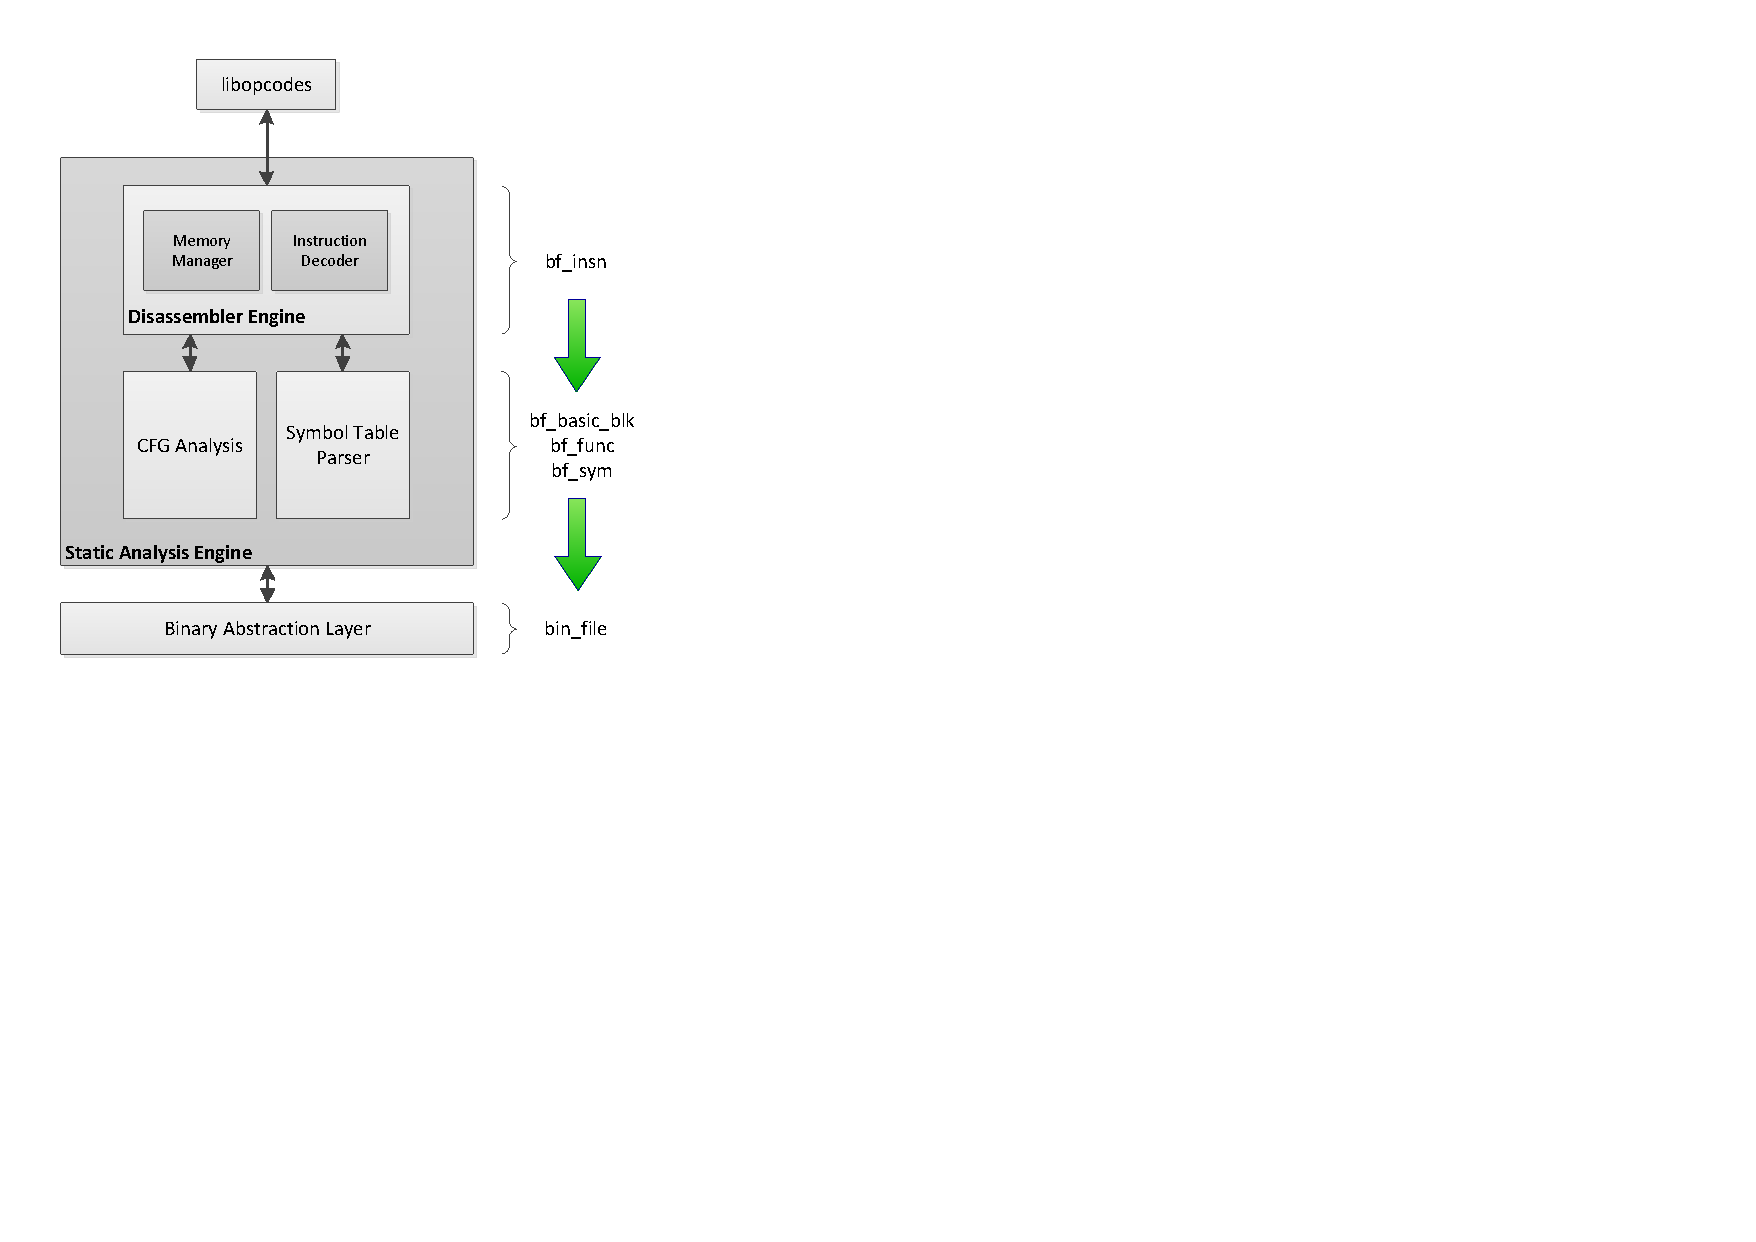
\includegraphics{Static_Analysis_Engine_Detail.pdf}
 \caption[Hierarchy]{The internal implementation of the static analysis engine.}
\label{fig:SAE_Detail}
\end{figure}

In order to understand how the static analysis engine works as a whole, we will explain each component in further detail.

\subsection{Disassembler Engine}

In practice, the disassembler engine is responsible for parsing and translating the strings received from libopcodes and storing the information in its internal semantic representation. At the most basic level, a \emph{bf\_insn} corresponds to an assembly instruction. In order to use libopcodes, we first needed to solve the two problems outlined in Design:

\begin{description}
\item [Limited disassembly scope] libopcodes can only disassemble a single address at a time which means the same applies for the disassembler engine. In order to make the disassembler engine useful, CFG analysis needs to be performed when an instruction is disassembled. The results of this analysis will then be used to drive the disassembler engine. For example, if the CFG analysis comes across a conditional branch instruction, it will need to instruct the disassembler engine to disassemble both the branch target and the next instruction. This analysis will be covered in detail later since it is not part of the disassembler engine.
\item [Output redirection] The default behaviour of libopcodes is to print to a stream using \emph{fprintf}. It is possible to override this behaviour by instructing libopcodes to invoke a custom function with the same prototype as fprintf.
\end{description}

One quirk of libopcodes is that it invokes the fprintf function (or overridden substitute) for each of the following `types': mnemonic, operand, separator and comment. As a concrete example, consider the following instruction:

\noindent\begin{minipage}{\textwidth}
\begin{lstlisting}[language={[x86masm]Assembler},caption={Example instruction disassembled by libopcodes.}]
ucomiss 0x9124(%rip), %xmm0 # 414d58
\end{lstlisting}
\end{minipage}

The custom fprintf function is invoked 4 times with the following:

\noindent\begin{minipage}{\textwidth}
\begin{lstlisting}[language={[x86masm]Assembler},caption={Strings received by custom fprintf. Type information is included for the benefit of the reader but is not given by libopcodes.}]
ucomiss (Mnemonic)
0x9124(%rip) (Operand)
, (Separator)
%xmm0 (Operand)
# (Separator)
414d58 (Comment)
\end{lstlisting}
\end{minipage}

One option is to concatenate all these instruction parts to obtain a full instruction but we already decided in Design that we would not store instructions in string form. Instead, the implementation stores semantic information about each instruction as it is disassembled by libopcodes. An issue with this is that libbind needs to know how to decode every type of string it receives. For example, an arbitrary string that is received might be a mnemonic, operand, separator or comment. It would be very inefficient to attempt to decode each string to determine what type it should be. libbind solves this issue by implementing a finite state machine which allows it to know what type it is expecting to receive:

\begin{figure}[H]
 \centering
 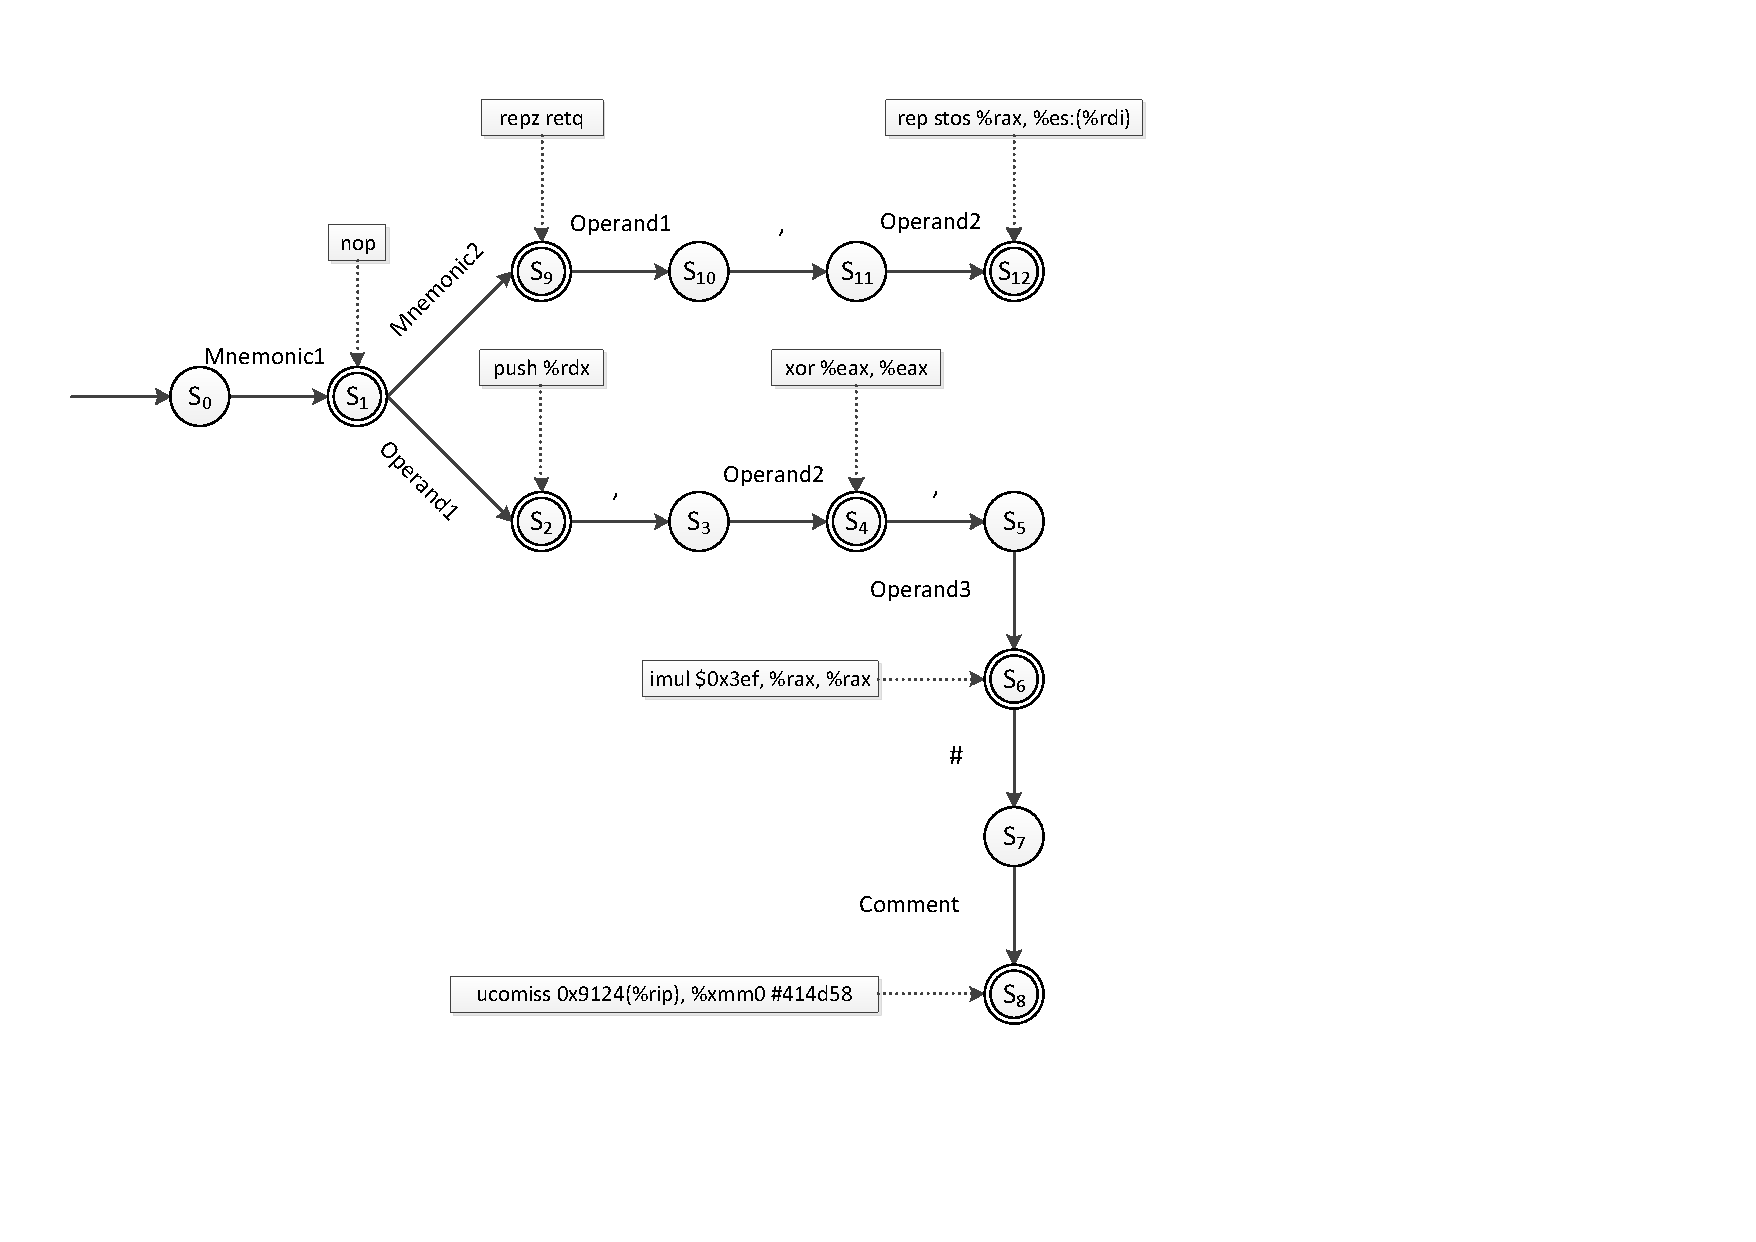
\includegraphics[scale=0.8]{Instruction_State_Machine.pdf}
 \caption[Hierarchy]{The instruction finite state machine used by the disassembler engine to determine how the received string should be decoded. A double circle denotes a possible terminal state. For each terminal state, an instruction which would cause termination at that state is shown.}
\label{fig:Instruction_State_Machine}
\end{figure}

\todo{This diagram might have to be redrawn to take up less horizontal space so it can be sized larger.}

Each time a new instruction is disassembled, a new bf\_insn object is constructed and the current state is restarted to the initial state of the instruction finite state machine. When fprintf is called, the received string is decoded based on its expected type, the semantic information updated for the bf\_insn and the current state of the state machine advanced. $S_1$ is a special case because two types can be received at this point: an operand or a mnemonic. In this case, we can only decode as one type and if that fails decode as the other type. Since an operand is more common, the disassembler engine attempts to decode as that first. The implementation of the instruction decoder is covered later.

\subsubsection{Memory Manager}

\subsubsection{Instruction Decoder}

\subsection{CFG Analysis}

\subsection{Symbol Table Parser}


%in practice, the disassembler engine is responsible for parsing and translating the strings received from libopcodes and storing that information in its internal semantic representation (bf\_insn, bf\_basic\_blk). bf\_func can be identified from three ways only:
%1) if it is the target of a call site
%2) if it corresponds to an address identified as a bf\_sym
%3) if the user defined it as a root for cfg generation and explicitly stated it is a function (cfg analysis and generation is covered in depth in...)
%
%further information such as size of symbols (which tells us size of function) is available because we are parsing the symbol table directly from libelf.
%
%quirks of libopcodes disassembler such as how it passes us the instruction parts (mnemonic, operands, separator) as strings! we build a finite state machine which allows us to 
%
%we can draw finite state machine in diagram here
%
%binary\_file
%
%within a binary\_file, there are 2 levels of code representation. firstly we have bf\_basic\_blk which represents a basic\_block as defined in architecture.
%
%binary\_file is composed of a CFG of bf\_basic\_blk objects. during the process of cfg generation and after it completes, we add extra information. i.e., bf\_func 'labels'
%
%bf\_func
%
%implementation of CFG analysis and generation...
%
%epilogue relocation

\section{Object File Injector}
\section{Static Patcher}

%
%distribution and documentation
%
%automake which we use to deal with library dependencies (libelf, libbfd, libopcodes, libkern).
%
% and doxygen
%
%WORKFLOW

%\chapter{Project Plan}

%If time permits, the most desirable extension is to add dynamic detouring to the library. %We would implement some form of runtime detouring and provide users with the option to %choose between both methods. Another smaller extension which would also be useful is to %allow the library to be invocable through the command-line as well as through the API (as %seen with ELFsh).